\documentclass{article}
\usepackage[utf8]{inputenc}
\usepackage[english]{babel}
\usepackage[]{amsthm} %lets us use \begin{proof}
\usepackage[]{amssymb} %gives us the character \varnothing
\usepackage{amsmath}
%\usepackage[shortlabels]{enumitem}
%\usepackage{CJKutf8}
\usepackage{float}
\usepackage{booktabs}
%\usepackage[hyperref]{acl2021}
%\usepackage{times}
%\usepackage{latexsym}

\title{ hqt part in final essay }
\author{Qitian (Jason) Hu}



\linespread{1}
\usepackage[margin=1.2in]{geometry}
\usepackage{graphicx}

\begin{document}
\maketitle 


\section{structural topic model}

The raw topic model (raw TM) only adds topic and document as internal organization of the corpus, but in practice, we usually have a much larger range of metadata. Structural topic modeling (sTM \cite{stm_sosc}) allows us to add document-level metadata on which topical prevalence or topical content is of interest. The main idea is to use generalized linear models as priors and then condition on metadata of the document. 

Based on three variants of LDA \cite{original_lda}, correlated topic model (CTM, \cite{blei2007correlated}), the Dirichlet-Multinomial Regression topic model (DMR, \cite{mimno2008topic}) and the Sparse Additive Generative (SAGE, \cite{taddy2013multinomial}) topic model.


 The logistic normal prior for topics in the standard CTM is replaced by a logistic-normal linear model. The design matrix for the covariates $X$ allows for flexible forms of the covariates that the prior could be conditioned on.
 
 The distribution over words is replaced with a multinomial logistic function such that a token's distribution is jointly determined by topic, covariates, and topic-covariate interaction. We adopted the R implementation provided by the authors \cite{stm_package}. 

 
 \begin{figure}[hbt]
  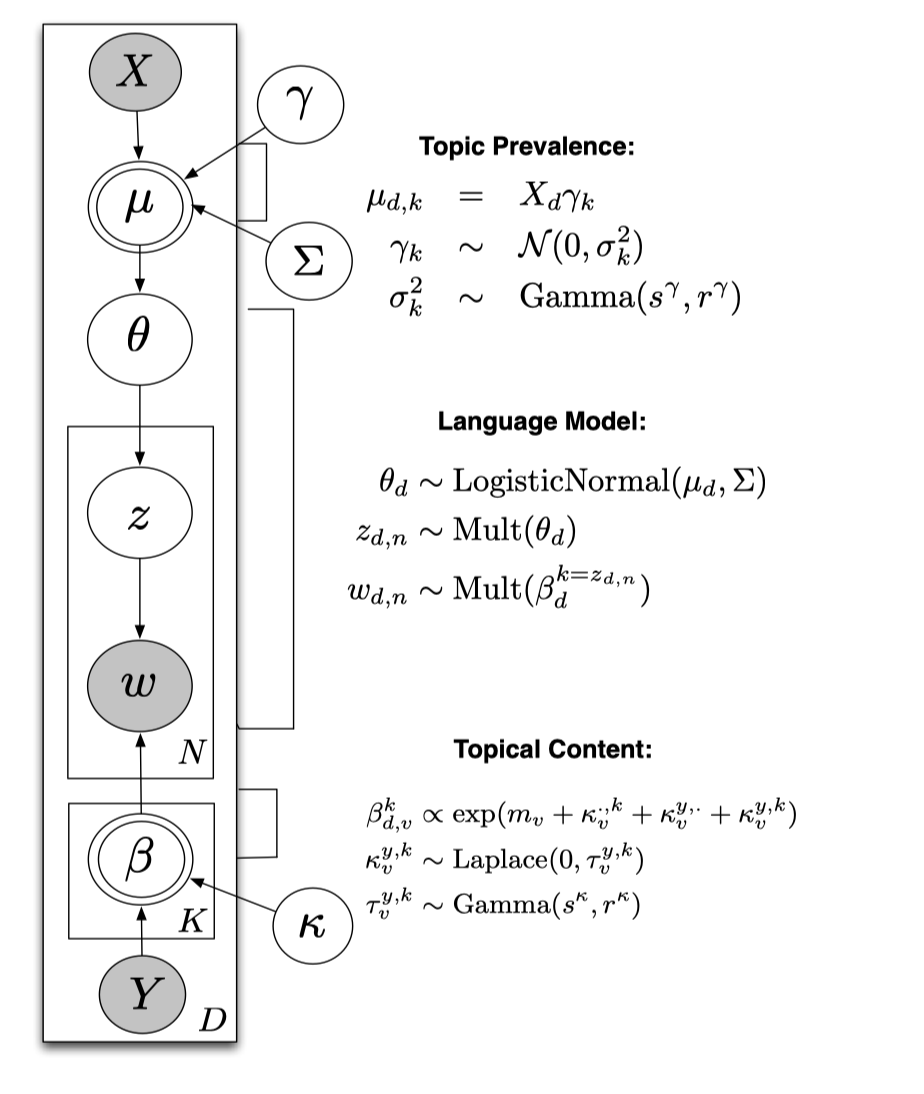
\includegraphics{pics/stm-explain-1.png}
  \caption{mechanism of structural topic model}
\end{figure}

 
 
 
 
A more specific description of the generative process is described here.

\begin{enumerate}
  \item Draw the document-level attention to each topic from a logistic-normal generalized linear model based on a vector of document covariates $X_{d}$.
$$
\vec{\theta}_{d} \mid X_{d} \gamma, \Sigma \sim \operatorname{Logistic} \operatorname{Normal}\left(\mu=X_{d} \gamma, \Sigma\right)
$$
where $X_{d}$ is a 1-by- $p$ vector, $\gamma$ is a $p$ -by- $K-1$ matrix of coefficients and $\Sigma$ is $K-1$ -by$K-1$ covariance matrix. 
  \item Given a document-level content covariate $y_{d}$, form the document-specific distribution over words representing each topic $(k)$ using the baseline word distribution $(m),$ the topic specific deviation $\kappa_{k}^{(\mathrm{t})},$ the covariate group deviation $\kappa_{y_{d}}^{(\mathrm{c})}$ and the interaction between the two $\left.\kappa_{y_{d}, k}^{(\mathrm{i})}\right)$
$$
\beta_{d, k} \propto \exp \left(m+\kappa_{k}^{(\mathrm{t})}+\kappa_{y_{d}}^{(\mathrm{c})}+\kappa_{y_{d}, k}^{(\mathrm{i})}\right)
$$
$m,$ and each $\kappa_{k}^{(\mathrm{t})}, \kappa_{y_{d}}^{(\mathrm{c})}$ and $\kappa_{y_{d}, k}^{(\mathrm{i})}$ are $V$ -length vectors containing one entry per word in the vocabulary. When no convent covariate is present $\beta$ can be formed as $\beta_{d, k} \propto$ $\exp \left(m+\kappa_{k}^{(\mathrm{t})}\right)$ or simply point estimated (this latter behavior is the default).

  \item For each word in the document, $\left(n \in 1, \ldots, N_{d}\right)$
- Draw word's topic assignment based on the document-specific distribution over topics.
$$
z_{d, n} \mid \vec{\theta}_{d} \sim \operatorname{Multinomial}\left(\vec{\theta}_{d}\right)
$$
- Conditional on the topic chosen, draw an observed word from that topic.
$$
w_{d, n} \mid z_{d, n}, \beta_{d, k=z_{d, n}} \sim \operatorname{Multinomial}\left(\beta_{d, k=z_{d, n}}\right)
$$


\end{enumerate}


\section{comparison between the two methods}

We choose to use People's Daily to compare the two topic models, because 
\begin{enumerate}
  \item The textual quality of the corpus is better
  \item It is large and thick enough to demonstrate the difference 
  \item It has a long time frame so structural topic model might be effective
\end{enumerate}

Although we used high-performance 128G-memory server, structural topic model could not be run probably, probably due to the limit of R language. Thus, we removed every word that appears in less than 10 documents or appear in more than half of all the documents. A brief comparison with the topics using the original corpus using raw topic model reveals that the quality of topics is not severely affected, and major historical themes are correctly identified. 

We compare raw topic model and structural topic from 3 aspects. Firstly, we interpretatively examine the topics and check if important historical themes are captured. We discovered that both models accurately captured the themes of anti-imperialism, Chairman Mao and cultural revolution, socialism and communism, United Nations and diplomacy, Korea and Vietnam wars, market economy, firm and investment, etc. sTM tends to capture more detailed topics, like Israel and Palestine, India and Pakistan, and municipal constructions, while these topics were not captured by raw TM. 

Secondly, to quantify the topic difference, we calculated the average number of characters of each word selected by the two topic models. Note that each Chinese word is composed by a number of characters, and usually the longer the word is, the more detailed and specific it is. The average word length for raw TM is 2.09 (std = 0.789), while that of sTM is 3.28 (std = 0.591). sTM tends to capture more detailed, specific words. 

Third, we visualize the time range of documents in each topic. As the figure shows, while raw TM tends to capture topics that capture documents around 1976, sTM topics could vary in the mean year of related documents. Time range of Raw TM topics have standard deviation centered at 17 year, while sTM topics could be very specific to a period (low standard deviation) or vice versa. 

To sum up, raw TM topics are more general and usually capture documents in a broader period. With metadata on the temporal change of prevalence of topics, sTM captures more specific topics of specific historical periods.



\section{Added Exploration}

\subsection{People's Daily Exploration}

People's Daily is the largest newspaper group in China, and is the official newspaper of the Central Committee of the Chinese Communist Party. It was founded in 1948 and represents the official ideology and policy of the Party. The corpus we we has about 1.3 million articles, ranging from 1948 until 2003. 

\subsubsection{Confirmation of Historical Knowledge}

We discovered that most of the fundamental shifts of the country's socio-intellectual history are accurately captured in the idea relations analysis. 

\begin{figure}[h!] 
  \centering
  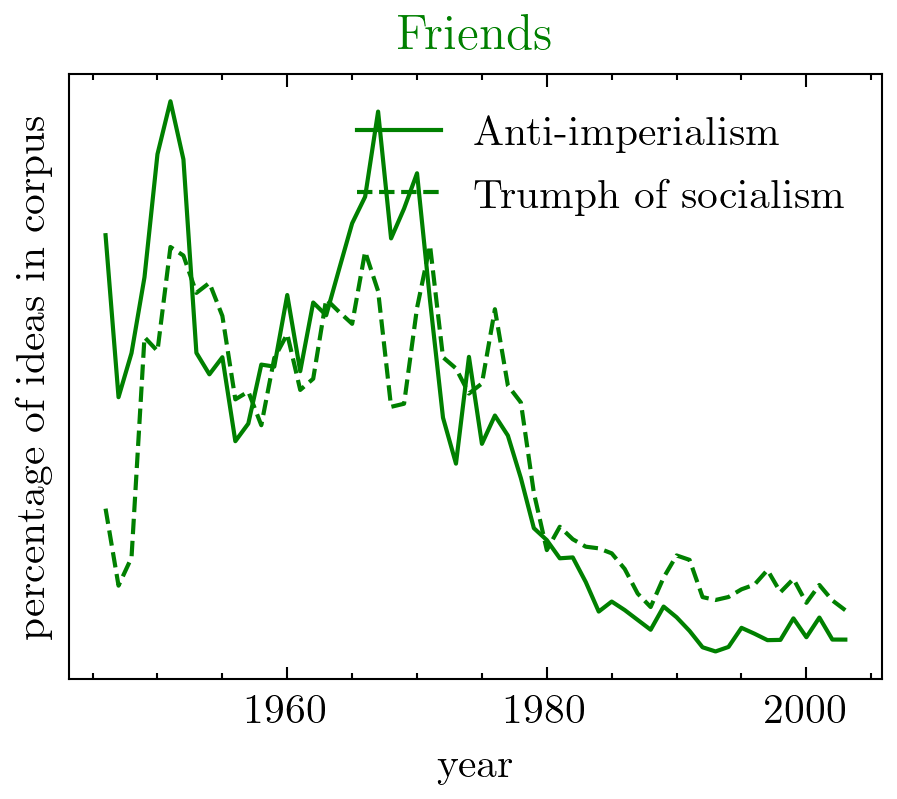
\includegraphics[scale=0.8]{acl-ijcnlp2021-templates/images/rmrb_1.png}
  \caption{Friends between Anti-imperialism and triumph of socialism}
  \label{fig:aer-arms}
\end{figure}


While China gradually transforms from an ideological nation to a more practical country aiming to for domestic economy, the prevalence of both the topic of anti-imperialism and the triumph of socialism declines. The friends relation also demonstrates that the triumph of socialism rhetoric is closely connected to the anti-imperialism argument, and the superiority of one's own ideology is shown by belittle the opponent ideology.

\begin{figure}[h!] 
  \centering
  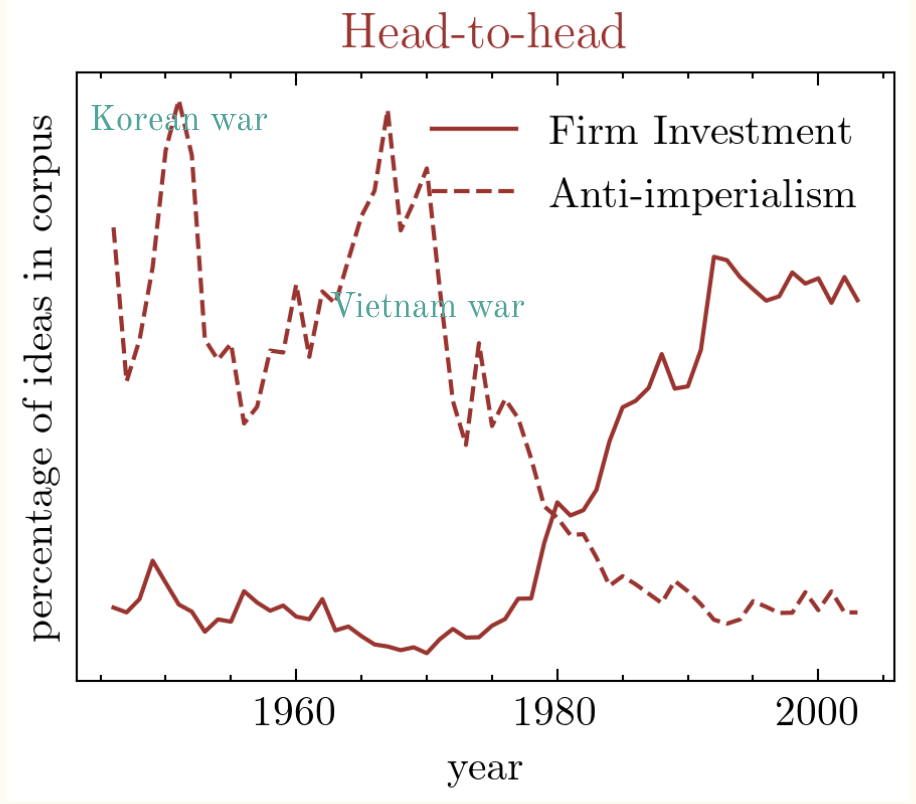
\includegraphics[scale=0.8]{acl-ijcnlp2021-templates/images/rmrb-new-2.png}
  \caption{Head-to-head between Anti-imperialism and Firm Investment}
  \label{fig:aer-arms}
\end{figure}


Transformation of the country is a double process: the decline of the revolutionary ideology and the rise of the economic rhetoric, and this figure perfects demonstrates this trend. Note that the two peaks of anti-imperialism topic correspond two important wars against the US, the Korean War and the Vietnam War; the official newspaper was also conducting an ideological campaign against the US. 

\begin{figure}[h!] 
  \centering
  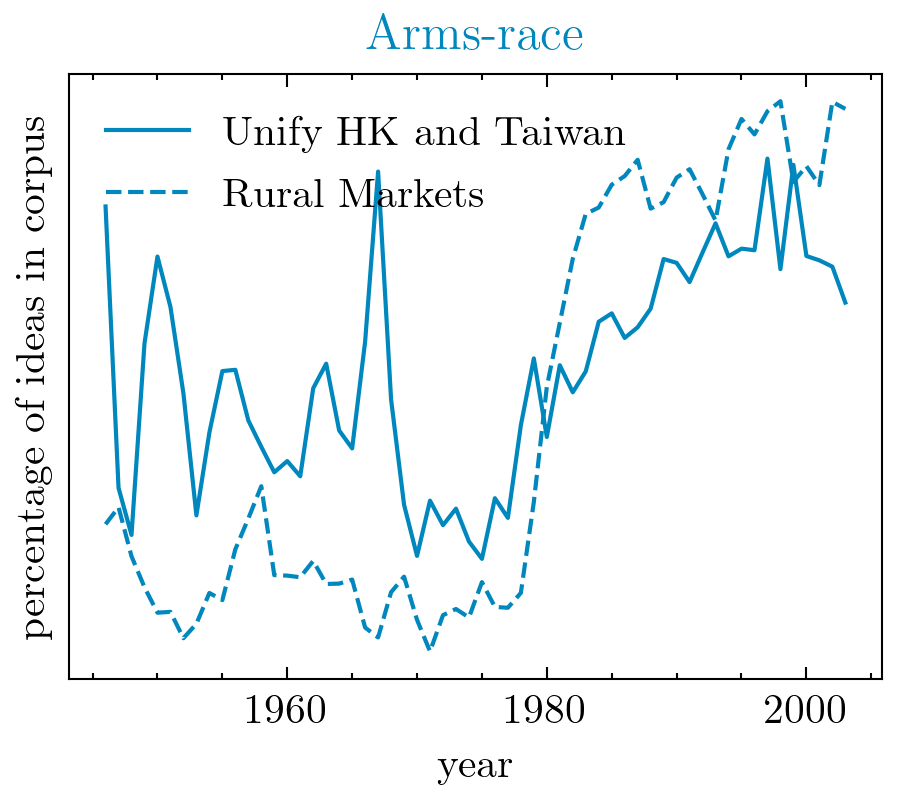
\includegraphics[scale=0.8]{acl-ijcnlp2021-templates/images/rmrb_6.png}
  \caption{Arms-race between Unify HK and Taiwan and Rural Markets}
  \label{fig:aer-arms}
\end{figure}

The topics of Unify HK and Taiwan and Rural Markets display similar trends in history, but seem to be unrelated in terms of the driving force behind, and this is accuratly captured by the lack of cooccurance. Unifying HK and Taiwan is an important theme throughout China's history, and it became important later in the timeframe because of specific events like Unification of HK and Taiwan Strait crisis and thus display a similar trend with the rural market topic, which is closely connected to the economic transformation of China.

\begin{figure}[h!] 
  \centering
  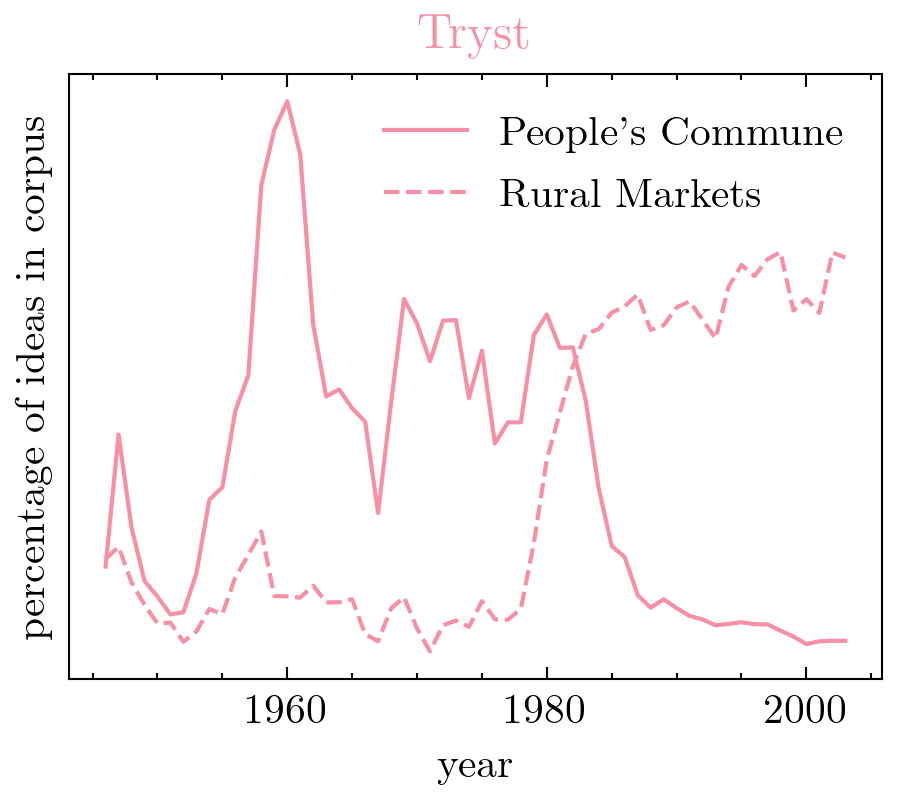
\includegraphics[scale=0.8]{acl-ijcnlp2021-templates/images/rmrb_7.png}
  \caption{Tryst between People's Commune and Rural Markets}
  \label{fig:aer-arms}
\end{figure}

People's Commune and Rural Markets are two distinct narratives on the same issue of rural economic development, and this explains their tendency to cooccur. However, the former is a derivative of Communism while the latter the result of the market-oriented reforms, and as the country transforms, the time trends of the two topics are opposite. 


\subsection{New Hypothesis}
The topic "diplomatic group visits" is consistently captured by the different algorithms and settings, and it is observed to be in a consistent arms-race with topics like People's Commune, Socialist construction, and other similar old, ideology-oriented ideas. It is unclear for now whether this is just driven by specific historical events or could be connected to more important themes in history, but hypothesis could be made for facilitate further exploration:

Hypothesis 1: diplomatic group in the Chinese context is an old-fashioned way of diplomacy and is sufficiently unrelated to  domestic development. 

Hypothesis 2: diplomatic group visits are usually reported in a special type of articles, and that type of articles are less published on People's Daily.




\section{further exploration}

Using structural topic models, we already observe interesting results on AER and People's Daily corpora, but further modifications could be made to facilitate research using the idea relations framework. 

\begin{enumerate}
  \item Different metadata. Like most real-life corpora, AER and People's Daily have numerous metadata available. For example, each People's Daily article has author, section, number of words, day in week, tone, etc. Adding these information as metadata in sTM could help us find more details in the historical ideas. 
  \item More textual information. With the goal to understand the change in PRC policy and ideology, we can add more text from other sources, like government announcements, other newspapers, and everyday writings of people. They could provide a more comprehensive view to the society while adding risks of mixing words with different connotations and thus making ideas illegible. 
  \item Combining the idea relations framework with causal inference. On the simple level, given the existing temporal structure of topics, we can locate concrete Granger causality and test them with historical knowledge or outside data. There are also other works exploring causal inference using texts \cite{causal1}, and it would be constructive to incorporate these ideas into ideas relations framework to allow more concrete social science knowledge to be produced.

\end{enumerate}





\section{Conclusion}

We replicated the ideas relations framework and extend it to the more flexible structural topic model, and also explored new datasets with the framework. We discovered insights in AER and People's Daily that correspond to our existing knowledge, and used the latter to make a detailed comparison and evaluation between the two topic models. We also demonstrate that the framework has the potential to facilitate the discovery of new historical knowledge. 

However, the explorations are interpretative in nature, and many of the topics and relations we discovered do not correspond to common knowledge, and it is difficult to distinguish whether they represent important trends in text and history, or they are just results of the randomness innate to our algorithm. It is also important to note that all discussion above should be viewed in the context of our corpus, which are just specific representations of the socio-historical trends we might be interested in.



We proposed a method to characterize relations between ideas in texts through the lens of cooccurrence within documents and prevalence correlation over time. For the first time, we observe that the distribution of pairwise cooccurrence is unimodal, while the distribution of pairwise prevalence correlation is not always unimodal, and show that they are positively correlated. This combination suggests four types of relations between ideas, and these four types are all found to varying extents in our experiments.

We illustrate our computational method by exploratory studies on news corpora and scientific research papers. We not only confirm existing knowledge but also suggest hypotheses around the usage of arab and islam in terrorism and latino and asian in immigration.

It is important to note that the relations found using our approach depend on the nature of the representation of ideas and the source of texts. For instance, we cannot expect relations found in news articles to reflect shifts in public opinion if news articles do not effectively track public opinion. Our method is entirely observational. It remains as a further stage of analysis to understand the underlying reasons that lead to these relations be-





Different types of metadata 

Adding other types of documents in corpus
Pro: comprehensive
Con: idea accuracy
Causal inference 
Granger causality 
Causal inference related to other real-world data 



















\bibliography{ours}
\end{document}